\documentclass[12pt, a4paper]{article}

% --- Packages ---
\usepackage[margin=2.5cm]{geometry}
\usepackage{amsmath, amssymb}
\usepackage{xcolor}
\usepackage{titlesec}
\usepackage{enumitem}
\usepackage{mdframed}
\usepackage{fontenc}
\usepackage{inputenc}
\usepackage{hyperref}
\usepackage{booktabs}
\usepackage{array}
\usepackage{parskip}
\usepackage{fancyhdr}
\usepackage{tcolorbox}
\usepackage{listings}
\usepackage{tikz}
\usetikzlibrary{arrows.meta, positioning, shapes.geometric, fit, backgrounds}

% --- Colours ---
\definecolor{theoryblue}{HTML}{1A3A5C}
\definecolor{theorybg}{HTML}{EAF1FB}
\definecolor{theoryborder}{HTML}{185FA5}
\definecolor{practicalgreen}{HTML}{0F4D2E}
\definecolor{practicalbg}{HTML}{E1F5EE}
\definecolor{practicalborder}{HTML}{0F6E56}
\definecolor{keyterm}{HTML}{534AB7}
\definecolor{stretchbg}{HTML}{FFF8E1}
\definecolor{stretchborder}{HTML}{BA7517}
\definecolor{delivbg}{HTML}{FDF3E3}
\definecolor{delivborder}{HTML}{BA7517}
\definecolor{codebg}{HTML}{F5F5F5}
\definecolor{codecomment}{HTML}{5C8A3C}
\definecolor{codekeyword}{HTML}{185FA5}
\definecolor{noteboxbg}{HTML}{F3F0FD}
\definecolor{noteboxborder}{HTML}{534AB7}
\definecolor{warnbg}{HTML}{FFF0F0}
\definecolor{warnborder}{HTML}{C0392B}

% --- Hyperref ---
\hypersetup{
  colorlinks=true,
  linkcolor=theoryblue,
  urlcolor=keyterm,
}

% --- Page style ---
\pagestyle{fancy}
\fancyhf{}
\rhead{\small\textcolor{gray}{AI Workflow Integration --- Self-Study Notes}}
\lhead{\small\textcolor{gray}{Day 2: Tool Use \& Function Calling}}
\cfoot{\small\thepage}
\renewcommand{\headrulewidth}{0.4pt}

% --- Section formatting ---
\titleformat{\section}{\large\bfseries\color{theoryblue}}{}{0em}{}[\titlerule]
\titleformat{\subsection}{\normalsize\bfseries\color{theoryblue}}{}{0em}{}
\titleformat{\subsubsection}{\normalsize\itshape\color{keyterm}}{}{0em}{}

% --- tcolorbox styles ---
\tcbuselibrary{skins, breakable}

\newtcolorbox{theorybox}[1][]{
  enhanced, breakable,
  colback=theorybg,
  colframe=theoryborder,
  coltitle=white,
  fonttitle=\bfseries\small,
  title={Theory --- 1 Hour},
  attach boxed title to top left={yshift=-2mm, xshift=4mm},
  boxed title style={colback=theoryborder, rounded corners},
  rounded corners, arc=4pt,
  left=6pt, right=6pt, top=10pt, bottom=6pt,
  #1
}

\newtcolorbox{practicalbox}[1][]{
  enhanced, breakable,
  colback=practicalbg,
  colframe=practicalborder,
  coltitle=white,
  fonttitle=\bfseries\small,
  title={ADK Hands-On --- 1 Hour},
  attach boxed title to top left={yshift=-2mm, xshift=4mm},
  boxed title style={colback=practicalborder, rounded corners},
  rounded corners, arc=4pt,
  left=6pt, right=6pt, top=10pt, bottom=6pt,
  #1
}

\newtcolorbox{notebox}{
  enhanced,
  colback=noteboxbg,
  colframe=noteboxborder,
  leftrule=3pt, toprule=0.4pt, bottomrule=0.4pt, rightrule=0.4pt,
  left=8pt, right=6pt, top=4pt, bottom=4pt,
  rounded corners, arc=2pt,
}

\newtcolorbox{warnbox}{
  enhanced,
  colback=warnbg,
  colframe=warnborder,
  leftrule=3pt, toprule=0.4pt, bottomrule=0.4pt, rightrule=0.4pt,
  left=8pt, right=6pt, top=4pt, bottom=4pt,
  rounded corners, arc=2pt,
}

\newtcolorbox{stretchbox}{
  enhanced,
  colback=stretchbg,
  colframe=stretchborder,
  leftrule=3pt, toprule=0.4pt, bottomrule=0.4pt, rightrule=0.4pt,
  left=8pt, right=6pt, top=4pt, bottom=4pt,
  rounded corners, arc=2pt,
}

\newtcolorbox{delivbox}{
  enhanced,
  colback=delivbg,
  colframe=delivborder,
  coltitle=delivborder,
  fonttitle=\bfseries\small,
  title={Day 2 Deliverable},
  attach boxed title to top left={yshift=-2mm, xshift=4mm},
  boxed title style={colback=delivbg, colframe=delivborder},
  rounded corners, arc=4pt,
  left=6pt, right=6pt, top=10pt, bottom=6pt,
}

% --- Code listings ---
\lstdefinestyle{bashstyle}{
  backgroundcolor=\color{codebg},
  basicstyle=\ttfamily\small,
  keywordstyle=\color{codekeyword}\bfseries,
  commentstyle=\color{codecomment}\itshape,
  stringstyle=\color{keyterm},
  breaklines=true,
  frame=single,
  framesep=4pt,
  rulecolor=\color{gray!30},
  xleftmargin=4pt,
  xrightmargin=4pt,
  showstringspaces=false,
}

\lstdefinestyle{pythonstyle}{
  backgroundcolor=\color{codebg},
  language=Python,
  basicstyle=\ttfamily\small,
  keywordstyle=\color{codekeyword}\bfseries,
  commentstyle=\color{codecomment}\itshape,
  stringstyle=\color{keyterm},
  breaklines=true,
  frame=single,
  framesep=4pt,
  rulecolor=\color{gray!30},
  xleftmargin=4pt,
  xrightmargin=4pt,
  showstringspaces=false,
  numbers=left,
  numberstyle=\tiny\color{gray},
  numbersep=5pt,
}

\lstdefinestyle{jsonstyle}{
  backgroundcolor=\color{codebg},
  basicstyle=\ttfamily\small,
  stringstyle=\color{keyterm},
  breaklines=true,
  frame=single,
  framesep=4pt,
  rulecolor=\color{gray!30},
  xleftmargin=4pt,
  xrightmargin=4pt,
  showstringspaces=false,
  morestring=[b]",
}

% --- Key term command ---
\newcommand{\kterm}[1]{\textbf{\textcolor{keyterm}{#1}}}

% ================================================================
% DOCUMENT
% ================================================================
\begin{document}

% --- Title block ---
\begin{center}
  {\small\textcolor{gray}{\textsc{AI Workflow Integration Specialist --- Self-Study Roadmap}}}\\[4pt]
  {\LARGE\bfseries\color{theoryblue} Day 2: Tool Use \& Function Calling}\\[6pt]
  {\small\textcolor{gray}{Week 1 $\cdot$ Google Agent Development Kit $\cdot$ Estimated time: 2 hours}}
\end{center}
\vspace{0.5em}
\hrule
\vspace{1.5em}

% ================================================================
% LEARNING OBJECTIVES
% ================================================================
\section{Learning Objectives}

By the end of Day 2 you should be able to:

\begin{enumerate}[leftmargin=*, label=\textbf{\arabic*.}]
  \item Explain how function calling APIs work at the protocol level and why they matter for agents.
  \item Write a well-formed function schema that the model can reason about reliably.
  \item Describe how an agent performs tool selection reasoning and what can go wrong.
  \item Define and produce structured JSON output from an agent using a schema.
  \item Implement at least three custom tools in ADK and wire them to an agent.
  \item Write and test deliberate edge cases that expose tool-call failure modes.
  \item Apply fallback strategies so tool failures do not crash the agent loop.
\end{enumerate}

\vspace{1.5em}

% ================================================================
% THEORY SECTION
% ================================================================
\begin{theorybox}

\subsection*{Chapter Focus: Tool-Use Patterns in Agentic Systems}

Yesterday's agent could only respond with text. Today it gains \emph{hands} --- the ability to call real functions, APIs, and services mid-loop. Tool use is the mechanism that makes agents genuinely useful in production.

% ---------------------------------------------------------------
\subsubsection*{How Function Calling APIs Work}

When you register a tool with an LLM, you are not giving the model direct access to your code. The protocol works in three phases:

\begin{center}
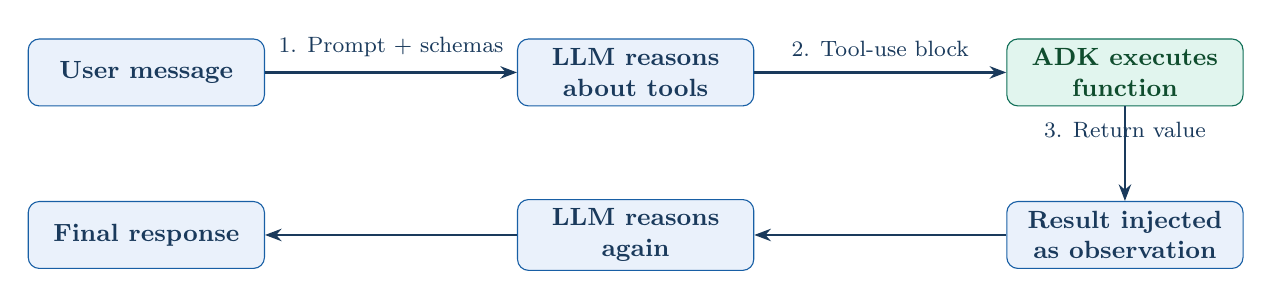
\begin{tikzpicture}[
  node distance=1.8cm and 3.2cm,
  box/.style={rectangle, rounded corners=4pt, draw=theoryborder, fill=theorybg,
               minimum width=3cm, minimum height=0.85cm, align=center,
               font=\small\bfseries\color{theoryblue}},
  sbox/.style={rectangle, rounded corners=4pt, draw=practicalborder, fill=practicalbg,
               minimum width=3cm, minimum height=0.85cm, align=center,
               font=\small\bfseries\color{practicalgreen}},
  arrow/.style={-{Stealth[length=6pt]}, thick, color=theoryblue},
  label/.style={font=\footnotesize\color{gray}, midway, above=2pt}
]
  \node[box] (user)   {User message};
  \node[box, right=of user] (llm1)   {LLM reasons\\about tools};
  \node[sbox, right=of llm1] (exec)   {ADK executes\\function};
  \node[box, below=1.2cm of exec] (obs)    {Result injected\\as observation};
  \node[box, left=of obs] (llm2)   {LLM reasons\\again};
  \node[box, left=of llm2] (resp)   {Final response};

  \draw[arrow] (user)  -- node[label]{1. Prompt + schemas} (llm1);
  \draw[arrow] (llm1)  -- node[label]{2. Tool-use block} (exec);
  \draw[arrow] (exec)  -- node[label]{3. Return value} (obs);
  \draw[arrow] (obs)   -- (llm2);
  \draw[arrow] (llm2)  -- (resp);
\end{tikzpicture}
\end{center}

\begin{enumerate}[leftmargin=*, itemsep=3pt]
  \item \textbf{Schema injection.} At the start of each turn, the model receives all registered tool schemas alongside the user message. It reads these as structured descriptions of what each function can do.
  \item \textbf{Tool-use block.} If the model decides a tool is needed, it \emph{does not} call it directly. Instead, it outputs a structured block (JSON) specifying the tool name and arguments. The ADK runtime intercepts this before the response reaches the user.
  \item \textbf{Observation injection.} ADK executes the function in Python, captures the return value, and injects it back into the conversation as a \emph{tool result} (also called an observation). The model then reasons again with this new context before producing the final user-facing response.
\end{enumerate}

\begin{notebox}
\textbf{Key insight:} The model never executes code. It only outputs a \emph{description} of what it wants to call and with what arguments. Your Python runtime does the actual execution. This separation is where all safety guarantees live.
\end{notebox}

% ---------------------------------------------------------------
\subsubsection*{Function Schemas}

A \kterm{function schema} is the contract between the model and your tool. It must answer three questions precisely: \emph{what does the tool do?}, \emph{what inputs does it need?}, and \emph{what does it return?}

In ADK, the schema is derived automatically from your Python function's docstring and type annotations. The model reads the docstring to decide \emph{when} to call the tool, and the type annotations to know \emph{how} to construct the arguments.

\medskip

\noindent\textbf{Anatomy of a well-formed schema:}

\begin{lstlisting}[style=jsonstyle, caption={JSON schema generated from a Python function}]
{
  "name": "get_exchange_rate",
  "description": "Converts an amount from one currency to another using
                  live exchange rates. Use this when the user asks about
                  currency conversion or exchange rates.",
  "parameters": {
    "type": "object",
    "properties": {
      "from_currency": {
        "type": "string",
        "description": "ISO 4217 currency code to convert from, e.g. USD"
      },
      "to_currency": {
        "type": "string",
        "description": "ISO 4217 currency code to convert to, e.g. NGN"
      },
      "amount": {
        "type": "number",
        "description": "The amount to convert. Must be positive."
      }
    },
    "required": ["from_currency", "to_currency", "amount"]
  }
}
\end{lstlisting}

\medskip

\noindent\textbf{Schema quality rules:}

\begin{itemize}[leftmargin=*, itemsep=2pt]
  \item The \texttt{description} field is the most important part. It is the model's only signal for deciding whether to call this tool. Write it as a usage instruction: ``Use this when\ldots''
  \item Parameter descriptions must be precise. ``ISO 4217 currency code'' is better than ``currency''. The model uses this to construct arguments correctly.
  \item Always declare \texttt{required} fields explicitly. Missing required parameters cause tool-call failures.
  \item Keep return values consistent. If the tool sometimes returns a string and sometimes a dict, the model will be confused. Standardise on a typed \texttt{dict}.
\end{itemize}

% ---------------------------------------------------------------
\subsubsection*{Tool Selection Reasoning}

When an agent has multiple tools available, it must decide at each reasoning step: \emph{do I need a tool at all, and if so, which one?} This is called \kterm{tool routing}.

The model performs this reasoning implicitly based on:

\begin{enumerate}[leftmargin=*, itemsep=2pt]
  \item \textbf{Semantic similarity} between the user's intent and each tool's description.
  \item \textbf{Argument availability} --- does the user's message contain the information needed to call this tool?
  \item \textbf{Prior context} --- what tools have already been called in this conversation?
\end{enumerate}

\noindent\textbf{Common routing failure modes:}

\begin{table}[h!]
\centering
\small
\begin{tabular}{>{\bfseries}p{3.5cm} p{4.5cm} p{4cm}}
\toprule
\textbf{Failure} & \textbf{Cause} & \textbf{Fix} \\
\midrule
Wrong tool selected & Overlapping descriptions & Rewrite descriptions to be mutually exclusive \\
\addlinespace
Tool called with wrong args & Ambiguous parameter names & Use precise names + examples in description \\
\addlinespace
Tool not called at all & Description too narrow & Broaden the ``Use this when'' clause \\
\addlinespace
Tool called in a loop & Ambiguous return value & Return a clear ``done'' or ``result'' key \\
\bottomrule
\end{tabular}
\caption{Tool routing failure modes and remedies}
\end{table}

% ---------------------------------------------------------------
\subsubsection*{Structured Output and JSON Schema}

\kterm{Structured output} means the agent is constrained to return a valid JSON object matching a predefined schema, rather than free-form prose. This is essential for any downstream system that needs to parse the agent's response programmatically.

\medskip

Two mechanisms exist:

\begin{enumerate}[leftmargin=*, itemsep=3pt]
  \item \textbf{Prompt-level enforcement.} Instruct the model in the system prompt to ``respond only in JSON matching this schema: \{\ldots\}''. Reliable for simple schemas; brittle for complex or nested ones.
  \item \textbf{Response schema parameter.} Pass a \texttt{response\_schema} argument to the model call. The model's sampling process is constrained to tokens that produce valid JSON matching the schema. More reliable but requires API support.
\end{enumerate}

\begin{notebox}
\textbf{Connection to Day 4--6:} The FinSight Agent's risk report is a structured JSON output. Every design decision you make today about schema quality will directly affect how cleanly that report generates at the end of the week.
\end{notebox}

% ---------------------------------------------------------------
\subsubsection*{Error Handling in Tool Calls}

Tool calls can fail for many reasons: network timeouts, invalid arguments, upstream API errors, or unexpected return types. An agent that crashes on the first tool failure is not production-ready.

\medskip

\noindent\textbf{Fallback strategies:}

\begin{description}[leftmargin=3.5cm, style=nextline, font=\bfseries\color{keyterm}]
  \item[Graceful degradation] The tool returns an error dict \texttt{\{"error": "message"\}} instead of raising an exception. The model reads this and decides to try a different tool or inform the user gracefully.
  \item[Retry with backoff] For transient failures (rate limits, timeouts), wrap the tool body in retry logic with exponential backoff before returning the result.
  \item[Fallback tool] Register a lower-quality fallback alongside the primary tool. If the primary fails, the model can route to the fallback instead.
  \item[Human escalation] For critical failures, the tool returns a sentinel value that triggers a human-in-the-loop step (relevant from Day 8 onwards).
\end{description}

% ---------------------------------------------------------------
\subsubsection*{Key Concepts Summary}

\begin{enumerate}[leftmargin=*, label=\textbf{\arabic*.}, itemsep=4pt]
  \item \kterm{Function schemas} --- the typed, described contract between the model and a Python function. Quality of the schema directly determines tool-call accuracy.

  \item \kterm{Tool routing} --- the model's implicit reasoning process for deciding which tool to invoke given the current context. Governed by description quality and argument availability.

  \item \kterm{Structured output} --- constraining the model's final response to a valid JSON object matching a predefined schema. Enables downstream parsing and system integration.

  \item \kterm{Fallback strategies} --- patterns for handling tool failures gracefully: error dicts, retries, fallback tools, and escalation mechanisms.
\end{enumerate}

\end{theorybox}

\vspace{1.5em}

% ================================================================
% PRACTICAL SECTION
% ================================================================
\begin{practicalbox}

\subsection*{Task: Build an Agent with 3+ Custom Tools}

Today you build a \textbf{multi-tool agent} and deliberately test its failure modes. The goal is not just to make tools work --- it is to understand what breaks and why.

\subsubsection*{Step 1 --- Project setup}

Create a new \texttt{day-2/} folder in your repository and initialise the structure:

\begin{lstlisting}[style=bashstyle]
mkdir day-2 && cd day-2
cp ../day-1/.env .          # reuse your API key file
touch multi_tool_agent.py
touch tools.py
touch README.md
\end{lstlisting}

\subsubsection*{Step 2 --- Define your three tools}

Each tool must have a precise docstring (this becomes the schema description), typed parameters, and a consistent return type. Below are three reference implementations. \textbf{You are encouraged to replace any of these with tools of your own choosing.}

\begin{lstlisting}[style=pythonstyle, caption={tools.py --- three custom tools with typed schemas}]
import math
import json
from datetime import datetime


# ----------------------------------------------------------------
# TOOL 1: Calculator
# ----------------------------------------------------------------
def calculate(expression: str) -> dict:
    """
    Evaluates a safe mathematical expression and returns the result.
    Use this when the user asks to compute, calculate, or evaluate
    any arithmetic expression. Examples: '2 + 2', '15% of 4000',
    'sqrt(144)'. Do NOT use for currency conversion.

    Args:
        expression: A mathematical expression as a string.

    Returns:
        A dict with 'result' (float) or 'error' (str).
    """
    try:
        # Restrict eval to math functions only — never exec user code
        allowed = {k: getattr(math, k) for k in dir(math) if not k.startswith("_")}
        allowed["__builtins__"] = {}
        result = eval(expression, allowed)  # noqa: S307
        return {"result": float(result), "expression": expression}
    except Exception as e:
        return {"error": str(e), "expression": expression}


# ----------------------------------------------------------------
# TOOL 2: Unit Converter
# ----------------------------------------------------------------
def convert_units(value: float, from_unit: str, to_unit: str) -> dict:
    """
    Converts a value between physical units (length, weight, temperature).
    Use this when the user asks to convert between km and miles, kg and
    lbs, Celsius and Fahrenheit, or similar unit conversions.
    Do NOT use for currency conversion.

    Args:
        value:     The numeric value to convert.
        from_unit: The source unit (e.g. 'km', 'kg', 'celsius').
        to_unit:   The target unit (e.g. 'miles', 'lbs', 'fahrenheit').

    Returns:
        A dict with 'result' (float) and 'unit' (str), or 'error' (str).
    """
    conversions = {
        ("km", "miles"):      lambda x: x * 0.621371,
        ("miles", "km"):      lambda x: x * 1.60934,
        ("kg", "lbs"):        lambda x: x * 2.20462,
        ("lbs", "kg"):        lambda x: x * 0.453592,
        ("celsius", "fahrenheit"): lambda x: (x * 9 / 5) + 32,
        ("fahrenheit", "celsius"): lambda x: (x - 32) * 5 / 9,
        ("meters", "feet"):   lambda x: x * 3.28084,
        ("feet", "meters"):   lambda x: x * 0.3048,
    }
    key = (from_unit.lower(), to_unit.lower())
    if key in conversions:
        return {
            "result": round(conversions[key](value), 4),
            "unit": to_unit,
            "original": f"{value} {from_unit}",
        }
    return {"error": f"Conversion from {from_unit} to {to_unit} is not supported."}


# ----------------------------------------------------------------
# TOOL 3: Timestamp Formatter
# ----------------------------------------------------------------
def format_timestamp(unix_timestamp: int, timezone_offset_hours: float = 0.0) -> dict:
    """
    Converts a Unix timestamp (seconds since epoch) to a human-readable
    date and time string. Use this when the user provides a numeric
    Unix timestamp and wants to know what date or time it represents.
    Optionally adjusts for a UTC offset.

    Args:
        unix_timestamp:       Seconds since Unix epoch (integer).
        timezone_offset_hours: UTC offset in hours, e.g. 1.0 for WAT (Lagos).

    Returns:
        A dict with 'formatted' (str), 'utc' (str), and 'local' (str).
    """
    try:
        utc_dt = datetime.utcfromtimestamp(unix_timestamp)
        offset_seconds = int(timezone_offset_hours * 3600)
        local_dt = datetime.utcfromtimestamp(unix_timestamp + offset_seconds)
        return {
            "utc":       utc_dt.strftime("%Y-%m-%d %H:%M:%S UTC"),
            "local":     local_dt.strftime("%Y-%m-%d %H:%M:%S"),
            "offset":    f"UTC+{timezone_offset_hours}",
            "formatted": local_dt.strftime("%A, %d %B %Y at %H:%M"),
        }
    except (OSError, OverflowError, ValueError) as e:
        return {"error": str(e), "unix_timestamp": unix_timestamp}
\end{lstlisting}

\subsubsection*{Step 3 --- Wire the tools into an ADK agent}

\begin{lstlisting}[style=pythonstyle, caption={multi\_tool\_agent.py --- agent with three registered tools}]
from google.adk.agents import Agent
from google.adk.runners import Runner
from google.adk.sessions import InMemorySessionService
from google.genai.types import Content, Part

from tools import calculate, convert_units, format_timestamp

# ----------------------------------------------------------------
# INIT — system prompt drives tool selection behaviour
# ----------------------------------------------------------------
SYSTEM_PROMPT = """
You are a precise utility assistant with access to three tools:
  - calculate:        for arithmetic and mathematical expressions
  - convert_units:    for physical unit conversions
  - format_timestamp: for converting Unix timestamps to readable dates

Always use a tool when the user's request maps to one. Never estimate
or calculate mentally — always call the appropriate tool. If a request
does not map to any available tool, say so clearly and explain why.

Return all tool results as structured data in your response.
"""

agent = Agent(
    name="multi_tool_agent",
    model="gemini-2.0-flash",
    instruction=SYSTEM_PROMPT,
    tools=[calculate, convert_units, format_timestamp],
)

session_service = InMemorySessionService()
runner = Runner(
    agent=agent,
    app_name="multi_tool_app",
    session_service=session_service,
)

# ----------------------------------------------------------------
# HELPER — send a message and print the response
# ----------------------------------------------------------------
def run(query: str, session_id: str = "session_1") -> str:
    message = Content(role="user", parts=[Part(text=query)])
    response_text = ""
    for event in runner.run(
        user_id="user_1",
        session_id=session_id,
        new_message=message,
    ):
        if event.is_final_response():
            response_text = event.response.parts[0].text
    return response_text


# ----------------------------------------------------------------
# TEST CASES — happy path + deliberate edge cases
# ----------------------------------------------------------------
if __name__ == "__main__":
    test_cases = [
        # Happy path
        ("Calculate sqrt(256) + 15% of 200",     "happy_calc"),
        ("Convert 100 km to miles",               "happy_units"),
        ("What date is Unix timestamp 1748000000?","happy_ts"),
        # Edge cases — observe how the agent handles these
        ("Convert 50 USD to NGN",                 "edge_currency"),   # no tool for this
        ("Calculate 10 / 0",                      "edge_divzero"),    # math error
        ("Convert 100 parsecs to light-years",    "edge_unsupported"),# unsupported units
        ("What is the timestamp for -9999999999?","edge_overflow"),   # overflow
    ]

    for query, session_id in test_cases:
        print(f"\n{'='*60}")
        print(f"Query   : {query}")
        print(f"Response: {run(query, session_id=session_id)}")
\end{lstlisting}

\subsubsection*{Step 4 --- Observe and document tool selection reasoning}

Run the agent and watch which tool gets chosen for each query. Pay attention to:

\begin{itemize}[leftmargin=*, itemsep=2pt]
  \item Does the agent call the right tool for each happy-path case?
  \item What does it do when no tool applies (the currency conversion edge case)?
  \item How does it respond to a tool that returns an \texttt{"error"} key instead of crashing?
  \item Does it ever call a tool with incorrect arguments?
\end{itemize}

Document your observations in \texttt{README.md} --- this is part of your Day 2 deliverable.

\begin{warnbox}
\textbf{Common failure to watch for:} The model may try to calculate a currency conversion using \texttt{calculate} with invented exchange rates rather than admitting it cannot do it. This is a hallucinated tool call --- the tool is misused to produce a plausible-looking but fabricated result. Note it if you observe it.
\end{warnbox}

\subsubsection*{Step 5 --- Add structured JSON output}

Modify your agent to enforce a structured response format. This prepares you directly for the FinSight risk report in Days 5--6.

\begin{lstlisting}[style=pythonstyle, caption={Enforcing structured output via response\_schema}]
import typing_extensions as typing

# Define the expected output shape using a TypedDict
class ToolResponse(typing.TypedDict):
    tool_used:   str    # name of the tool called, or "none"
    input_query: str    # the user's original query
    result:      str    # human-readable result
    raw_output:  dict   # the dict returned by the tool

# Pass the schema to the agent
agent_structured = Agent(
    name="structured_tool_agent",
    model="gemini-2.0-flash",
    instruction=SYSTEM_PROMPT + "\n\nAlways respond in the specified JSON schema.",
    tools=[calculate, convert_units, format_timestamp],
    output_schema=ToolResponse,
    output_key="tool_response",
)
\end{lstlisting}

\subsubsection*{Step 6 --- Stretch goal: log tool selection reasoning}

Add a callback that prints which tool was selected and the model's reasoning before each tool call is executed. In ADK, this is done via event inspection in the run loop:

\begin{lstlisting}[style=pythonstyle, caption={Extracting tool-call reasoning from the event stream}]
for event in runner.run(
    user_id="user_1",
    session_id="debug_session",
    new_message=Content(role="user", parts=[Part(text="Convert 5 kg to lbs")]),
):
    # Inspect intermediate events (tool calls) before the final response
    if hasattr(event, "content") and event.content:
        for part in event.content.parts:
            # Tool-use parts reveal what the model decided to call
            if hasattr(part, "function_call") and part.function_call:
                fc = part.function_call
                print(f"[TOOL SELECTED] {fc.name}")
                print(f"[ARGUMENTS]     {dict(fc.args)}")
            # Tool-result parts show what came back
            if hasattr(part, "function_response") and part.function_response:
                fr = part.function_response
                print(f"[TOOL RESULT]   {fr.response}")

    if event.is_final_response():
        print(f"[FINAL RESPONSE] {event.response.parts[0].text}")
\end{lstlisting}

\subsubsection*{Step 7 --- Commit to GitHub}

\begin{lstlisting}[style=bashstyle]
cd ..   # back to repo root
git add day-2/
git commit -m "Day 2: multi-tool agent with 3 tools + edge case docs"
git push
\end{lstlisting}

\medskip

\begin{stretchbox}
\textbf{Stretch Goal:} Extend the logging from Step 6 to write a structured JSON log file (\texttt{tool\_call\_log.json}) after each run. Each entry should record: timestamp, query, tool selected, arguments passed, tool return value, and the model's final response. This is the embryo of the evaluation harness you will build on Day 6.
\end{stretchbox}

\end{practicalbox}

\vspace{1.5em}

% ================================================================
% DELIVERABLE
% ================================================================
\begin{delivbox}
\begin{itemize}[leftmargin=*, itemsep=3pt]
  \item Multi-tool agent with at least 3 custom tools committed to \texttt{day-2/} on GitHub.
  \item All happy-path test cases passing and producing correct results.
  \item At least one edge case documented in \texttt{README.md}: describe what you tested, what the agent did, and whether the behaviour was correct.
  \item (Stretch) Tool selection log written to \texttt{tool\_call\_log.json} for at least 5 queries.
\end{itemize}
\end{delivbox}

\vspace{1.5em}

% ================================================================
% SELF-CHECK QUESTIONS
% ================================================================
\section{Self-Check Questions}

\begin{enumerate}[leftmargin=*, label=\textbf{Q\arabic*.}, itemsep=6pt]
  \item Walk through the three phases of a function call cycle. At which phase does your Python code actually execute?
  \item You have two tools: \texttt{search\_web} and \texttt{search\_database}. A user asks to ``look up the current price of gold.'' The model keeps calling \texttt{search\_database}. What is most likely wrong and how do you fix it?
  \item What is the difference between prompt-level structured output enforcement and response schema enforcement? When would you prefer one over the other?
  \item Why should a tool return \texttt{\{"error": "message"\}} instead of raising a Python exception? What happens to the agent loop if an exception propagates?
  \item What is a hallucinated tool call? Give an example and explain why it is dangerous in a production system.
  \item You notice the agent is calling \texttt{calculate} with the string \texttt{"10 USD in NGN"} as the expression. What does this reveal about your tool descriptions, and how do you fix it?
\end{enumerate}

\vspace{1.5em}

% ================================================================
% CONNECTIONS TO THE BROADER ROADMAP
% ================================================================
\section{Connections to the Broader Roadmap}

\begin{table}[h!]
\centering
\small
\begin{tabular}{>{\bfseries}p{2.5cm} p{4.5cm} p{5cm}}
\toprule
\textbf{Today} & \textbf{This leads to\ldots} & \textbf{Why it matters} \\
\midrule
Function schemas & Day 4--6: FinSight sub-agents & Every sub-agent in FinSight exposes tools to the orchestrator using the same schema pattern. \\
\addlinespace
Tool routing & Day 5: ReAct reasoning loops & ReAct explicitly models the thought-action-observation cycle you observed today. \\
\addlinespace
Structured output & Day 5--6: JSON risk reports & The \texttt{ToolResponse} schema you defined today is a prototype for the FinSight report schema. \\
\addlinespace
Error handling & Day 6: Evaluation harness & Graceful error dicts are what allow an eval harness to classify failures programmatically. \\
\addlinespace
Tool call logging & Day 6: Observability & The JSON log from today's stretch goal is the first version of a trace --- the backbone of Day 6. \\
\bottomrule
\end{tabular}
\caption{How Day 2 concepts thread through the sprint}
\end{table}

% ================================================================
% QUICK REFERENCE
% ================================================================
\section{Quick Reference}

\subsection*{Glossary}

\begin{description}[leftmargin=4cm, style=nextline, font=\bfseries\color{keyterm}]
  \item[Function schema] The typed, described contract between the model and a tool: name, description, parameter names/types, and required fields.
  \item[Tool routing] The model's implicit reasoning process for selecting which tool to invoke, based on description matching and argument availability.
  \item[Tool-use block] The structured JSON output produced by the model when it decides to call a tool, before any Python code runs.
  \item[Observation] The tool's return value, injected back into the conversation context for the model's next reasoning step.
  \item[Structured output] A model response constrained to a valid JSON object matching a predefined schema.
  \item[Fallback strategy] A pattern for handling tool failures: error dicts, retries, fallback tools, or human escalation.
  \item[Hallucinated tool call] When the model misuses an available tool to produce a plausible-looking but fabricated result for a query the tool was not designed to handle.
  \item[output\_schema] An ADK Agent parameter that constrains the model's response to a specific typed schema.
  \item[function\_call part] An event part in the ADK run loop that reveals which tool the model selected and with what arguments, before execution.
\end{description}

\subsection*{Schema Quality Checklist}

Before registering any tool, verify:

\begin{itemize}[leftmargin=*, itemsep=2pt]
  \item[$\square$] Docstring starts with a one-line summary of what the tool does.
  \item[$\square$] Docstring includes a ``Use this when\ldots'' clause that distinguishes it from similar tools.
  \item[$\square$] All parameters have type annotations (\texttt{str}, \texttt{float}, \texttt{int}, etc.).
  \item[$\square$] Parameter docstrings include examples where the format is non-obvious.
  \item[$\square$] Return type is always a \texttt{dict} with consistent keys.
  \item[$\square$] All failure paths return \texttt{\{"error": str\}} rather than raising exceptions.
\end{itemize}

\subsection*{Key ADK Patterns Today}

\begin{lstlisting}[style=pythonstyle]
# Register tools at agent init
agent = Agent(name="...", model="...", instruction="...",
              tools=[tool_1, tool_2, tool_3])

# Enforce structured output
agent = Agent(..., output_schema=MyTypedDict, output_key="result")

# Inspect tool calls in the event stream
for event in runner.run(...):
    for part in (event.content.parts if event.content else []):
        if hasattr(part, "function_call") and part.function_call:
            print(part.function_call.name, dict(part.function_call.args))
\end{lstlisting}

\vfill
\noindent\rule{\textwidth}{0.4pt}\\
{\small\textcolor{gray}{AI Workflow Integration Specialist --- Week 1 Study Notes \hfill Day 2 of 14}}

\end{document}
